\documentclass{ximera}

%% Where to look for inputs
\makeatletter     %% make "@" a letter-character
\def\input@path{  %% When looking for files,
{./}              %% look first at your level
{./coverArt/}     %% then in this folder,
{./introduction/} %% then in this folder,
}
\makeatother      %% make "@" an other-character

%% Where to find images
\graphicspath{                      %% When looking for images, 
{./}                                %% look first at your level,
{./setup/}                          %% then in this folder,
{./graphicsVideosAndInteractives/}  %% then in this folder,
}



% Custom Commands


%% These may change and should be checked! 
\newcommand{\docURL}{\url{https://github.com/ximeraProject/ximeraFirstSteps/ximeraUserManual}}
\newcommand{\testURL}{\url{https://github.com/ximeraProject/tests}}
\newcommand{\experimentalURL}{\url{https://github.com/ximeraProject/experimental}}
\newcommand{\xfsURL}{https://go.osu.edu/xfs}
\newcommand{\xfgURL}{https://go.osu.edu/ximera-flash-grant}

\newcommand{\event}[1]{\def\theevent{#1}}
\newcommand{\theevent}{}


\newif\ifcolor %% for color cover
\colorfalse
\colorlet{bkgndcr}{white}
\colorlet{txtcr}{black}
\colorlet{otherbkgndcr}{white}
\colorlet{othertxtcr}{black}


\usepackage{qrcode} %% For QR Codes
\usepackage[normalem]{ulem} % for strikeout
\usepackage{multicol} % multicols -- PDF only

\makeatletter
%% Make Front style
\newcommand\frontstyle{%
  \def\activitystyle{activity-chapter}
  \def\maketitle{%
                {\flushleft\small\sffamily\bfseries\@pretitle\par\vspace{-1.5em}}%
                {\flushleft\LARGE\sffamily\bfseries\@title \par }%3
                {\vskip .6em\noindent\textit\theabstract\setcounter{problem}{0}\setcounter{section}{0}}%
                \par\vspace{2em}    
                \phantomsection\addcontentsline{toc}{section}{\textbf{\@title}}%
                \setcounter{titlenumber}{0}
}}

\renewcommand\chapterstyle{%
  \def\activitystyle{activity-chapter}
  \normalsize
  %\onecolumn
  \def\maketitle{%
    \addtocounter{titlenumber}{1}%
                    {\flushleft\small\sffamily\bfseries\@pretitle\par\vspace{-1.5em}}%
                    {\flushleft\LARGE\sffamily\bfseries\thetitlenumber\hspace{1em}\@title \par }%
                    {\vskip .6em\noindent\textit\theabstract\setcounter{problem}{0}\setcounter{section}{0}}%
                    \par\vspace{2em}
                    \phantomsection\addcontentsline{toc}{section}{\textbf{\thetitlenumber\hspace{1em}\@title}}%
}}

%% Redefine section and subsection
\renewcommand\section{\@startsection {section}{1}{\z@}%
                                   {-3.5ex \@plus -1ex \@minus -.2ex}%
                                   {2.3ex \@plus.2ex}%
                                   {\boldmath\normalfont\large\bfseries\sffamily}}
\renewcommand\subsection{\@startsection{subsection}{2}{\z@}%
                                     {-3.25ex \@plus -1ex \@minus -.2ex}%
                                     {1.5ex \@plus .2ex}%
                                     {\boldmath\normalfont\large\bfseries\sffamily}}


\renewcommand\paragraph{\@startsection{paragraph}{4}{\z@}%
                                    {3.25ex \@plus1ex \@minus.2ex}%
                                    {-1em}%
                                    {\boldmath\normalfont\normalsize\bfseries\sffamily}}
\makeatother

\title{Preambles, input paths, and graphics paths}

\author{Bart Snapp}

\begin{document}
\begin{abstract}
  How to add extra packages and commands
\end{abstract}
\maketitle



The Ximera documentclass comes with many packages preloaded:
\verb!enumitem!, 
\verb!titlesec!, 
\verb!titletoc!, 
\verb!titling!, 
\verb!url!, 
\verb!xcolor!, 
\verb!tikz!, 
\verb!pgfplots!, 
\verb!fancyvrb!, 
\verb!forloop!, 
\verb!environ!, 
\verb!amssymb!, 
\verb!amsmath!, 
\verb!amsthm!, 
\verb!xifthen!, 
\verb!multido!, 
\verb!listings!, 
\verb!xkeyval!, 
\verb!comment!, 
\verb!gettitlestring!, 
\verb!nameref!, 
\verb!epstopdf!, 
\verb!hyperref!.

The documentclass also provides support for the following theorem-like
environments:
\verb!algorithm!, \verb!axiom!, \verb!claim!, \verb!conclusion!,
\verb!condition!, \verb!conjecture!, \verb!corollary!, \verb!criterion!,
\verb!definition!, \verb!example!, \verb!explanation!, \verb!exercise!,
\verb!exploration!,
\verb!fact!, \verb!formula!, \verb!hypothesis!, \verb!idea!, \verb!lemma!,
\verb!model!,
\verb!notation!, \verb!observation!, \verb!paradox!, \verb!proof!, \verb!problem!,
\verb!procedure!,
\verb!proposition!, \verb!question!, \verb!remark!, \verb!solution!,
\verb!summary!, \verb!template!, \verb!theorem!, \verb!warning!.


We can add functionality and generality, via user defined commands, to the document via a preamble, or macros, document. 
The purpose of a preamble is to ensure \textbf{all files compile consistently,
  it is not for cosmetic changes.} A typically preamble might contain things
like:

\begin{verbatim}
\newcommand{\R}{\mathbb{R}}
\newcommand{\d}{\, d}
\end{verbatim}

\begin{warning}
  Cosmetic changes to Ximera environments will result in unpredictable behavior
  online.
\end{warning}

Since every \verb!*.tex! file with a \verb!\documentclass! must compile, the preamble file must be accessible  by all files.
\begin{center}%%DIAGRAM OF FILE STRUCTURE
  \scalebox{.7}{
    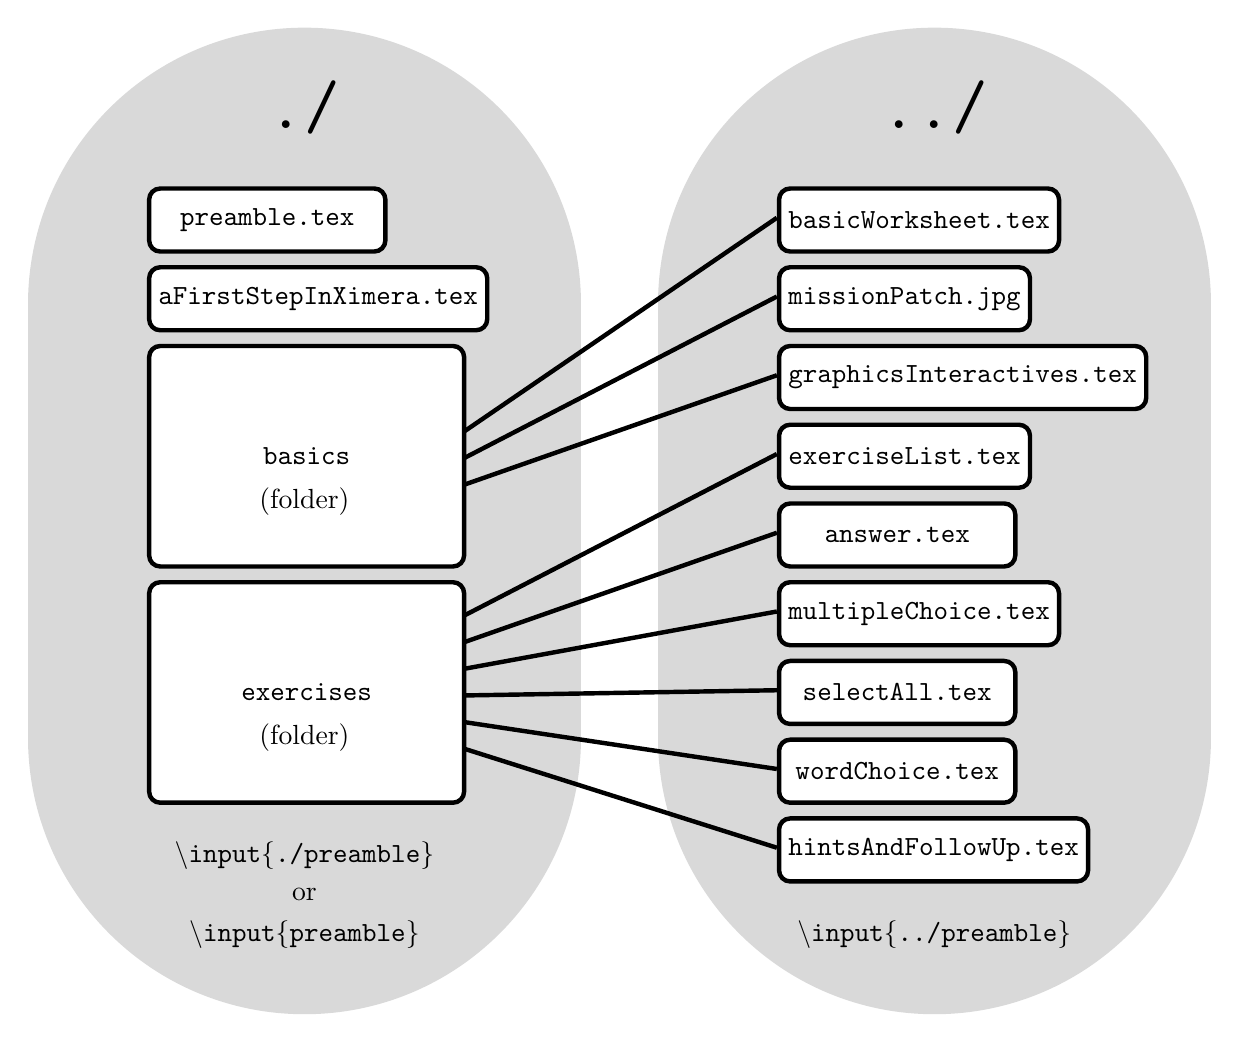
\begin{tikzpicture}
      % Define styles for nodes
      \tikzstyle{document} = [anchor=north west,draw, rounded corners,
      rectangle,
      minimum width=3cm,fill=white, minimum height=.8cm, ultra
      thick,font=\ttfamily]
      \tikzstyle{folder} = [anchor=north west,draw, rectangle, rounded corners,
      minimum width=4cm,fill=white, minimum height=2.8cm, ultra
      thick,font=\ttfamily]

      % Thick grey lines
      \draw[line width=200pt,white!85!black,line cap=round] (2,1.5) -- (2,-4);
      \draw[line width=200pt,white!85!black,line cap=round] (10,1.5) --
      (10,-4);

      % Connections
      \draw[ultra thick] (2,-1.5) -- (8,2.6);
      \draw[ultra thick] (2,-1.5) -- (8,1.6);
      \draw[ultra thick] (2,-1.5) -- (8,.6);

      \draw[ultra thick] (2,-3.5) -- (8,-.4);
      \draw[ultra thick] (2,-3.5) -- (8,-1.4);
      \draw[ultra thick] (2,-3.5) -- (8,-2.4);
      \draw[ultra thick] (2,-3.5) -- (8,-3.4);
      \draw[ultra thick] (2,-3.5) -- (8,-4.4);
      \draw[ultra thick] (2,-3.5) -- (8,-5.4);

      % Symbols at top
      \node at (2,4) {\Huge \tt ./};
      \node at (10,4) {\Huge \tt ../};

      % Define the folders at top level
      \node[document] at (0,3) {preamble.tex};
      \node[document] at (0,2) {aFirstStepInXimera.tex};
      \node[folder] at (0,1) {basics};
      \node[] at (2,-1) {(folder)};
      \node[folder] at (0,-2) {exercises};
      \node[] at (2,-4) {(folder)};

      % Define the documents in the basics folder
      \node[document] at (8,3) {basicWorksheet.tex};
      \node[document] at (8,2) {missionPatch.jpg};
      \node[document] at (8,1) {graphicsInteractives.tex};

      % Define the documents in the exercises folder
      \node[document] at (8,0) {exerciseList.tex};
      \node[document] at (8,-1) {answer.tex};
      \node[document] at (8,-2) {multipleChoice.tex};
      \node[document] at (8,-3) {selectAll.tex};
      \node[document] at (8,-4) {wordChoice.tex};
      \node[document] at (8,-5) {hintsAndFollowUp.tex};

      % paths at bottom
      \node at (2,-5.5) {\tt\textbackslash input\{./preamble\}};
      \node at (2,-6) {or};
      \node at (2,-6.5) {\tt\textbackslash input\{preamble\}};
      \node at (10,-6.5) {\tt\textbackslash input\{../preamble\}};
    \end{tikzpicture}}
\end{center}
In this diagram, we attempt to show how one should modify the inputs of the
preamble based on the directory structure.

\paragraph{Graphics paths} help \verb!\xourse! files find images. 
We used \verb!\includegraphics! in \texttt{basicWorkSheet.tex} with code like:
\begin{verbatim} 
\begin{center}
  
\includegraphics[width=5cm]{missionPatch.jpg}
\end{center}
\end{verbatim}
In this case, \texttt{basicWorkSheet.tex}  and \verb!missionPatch.jpg! are both in the folder
\texttt{basics}. However, when
this document is compiled via a \verb!xourse! document, the \LaTeX\ compiler
looks for the image \textit{at the level of the
  \texttt{aFirstStepInXimera.tex}}.
\begin{center}%%DIAGRAM OF FILE STRUCTURE
  \scalebox{.7}{
    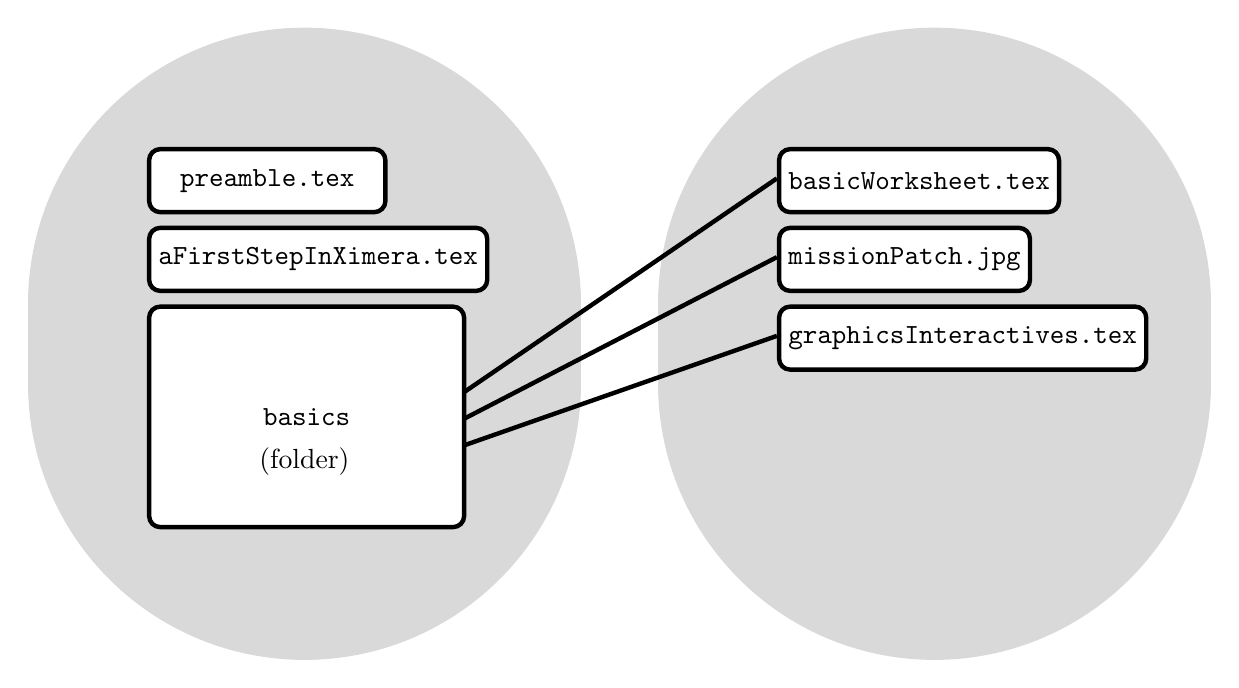
\begin{tikzpicture}
      % Define styles for nodes
      \tikzstyle{document} = [anchor=north west,draw, rounded corners,
      rectangle,
      minimum width=3cm,fill=white, minimum height=.8cm, ultra
      thick,font=\ttfamily]
      \tikzstyle{folder} = [anchor=north west,draw, rectangle, rounded
      corners,
      minimum width=4cm,fill=white, minimum height=2.8cm, ultra
      thick,font=\ttfamily]

      % Thick grey lines
      \draw[line width=200pt,white!85!black,line cap=round] (2,0) -- (2,1);
      \draw[line width=200pt,white!85!black,line cap=round] (10,0)--(10,1);

      % Connections
      \draw[ultra thick] (2,-1.5) -- (8,2.6);
      \draw[ultra thick] (2,-1.5) -- (8,1.6);
      \draw[ultra thick] (2,-1.5) -- (8,.6);

      % Define the folders at top level
      \node[document] at (0,3) {preamble.tex};
      \node[document] at (0,2) {aFirstStepInXimera.tex};
      \node[folder] at (0,1) {basics};
      \node[] at (2,-1) {(folder)};

      % Define the documents in the basics folder
      \node[document] at (8,3) {basicWorksheet.tex};
      \node[document] at (8,2) {missionPatch.jpg};
      \node[document] at (8,1) {graphicsInteractives.tex};

    \end{tikzpicture}}
\end{center}
Since there is no file \verb!missionPatch.jpg! (which is on the right) at the
level of the
\verb!xourse! document (on the left) the compilation will fail. To solve this
problem we use the preamble to append the graphics path. If we add (and in
reality we did!) this
\begin{verbatim}
%% Where to find images
\graphicspath{  %% When looking for images,
{./}            %% look first at your level,
{./basics/}     %% then in this folder,
}    
\end{verbatim}
to our preamble, then when compiling \verb!aFirstStepInXimera.tex!, the
compiler will know where to look.

\paragraph{Input paths} allow you to load other documents into your files. 
This is a less common use case, but we'll mention it here. You can surely avoid the use of such files with an enhanced preamble. However, for this document, we
needed to input various TikZ files to help us draw our diagrams. Hence we needed to
add the location of these files to our input path. We did this in our preamble
the following way:
\begin{verbatim}
%% Where to look for inputs
\makeatletter     %% make "@" a letter-character
\def\input@path{  %% When looking for files,
{./}              %% look first at your level
{./coverArt/}     %% then in this folder,
{./introduction/} %% then in this folder,
}
\makeatother      %% make "@" an other-character
\end{verbatim}
With this said, modifying input paths is more of an advanced feature and one should be careful.
\end{document}
